\documentclass[12pt,oneside]{report}
\usepackage[left=1.5in,right=1in,top=1.25in,bottom=1.25in]{geometry}
\IfFileExists{mathptmx.sty}{\usepackage{mathptmx}}{}
\usepackage{booktabs}
\usepackage{longtable}
\usepackage{array}
\usepackage{graphicx}
\usepackage{hyperref}
\usepackage{enumitem}
\usepackage{setspace}
\usepackage{caption}
\usepackage{float}
\usepackage{xcolor}
\usepackage{url}
\usepackage{tocloft}
\usepackage{etoolbox}
\usepackage{amsmath}
\usepackage{titlesec}
\hypersetup{colorlinks=true,linkcolor=blue,citecolor=blue,urlcolor=blue}
\doublespacing
\pagestyle{plain}
\setlength{\parindent}{0.5in}
\setlength{\parskip}{0pt}
\graphicspath{{latex/figures/generated/}{latex/figures/manual/}}
\captionsetup{font=small}
\titleformat{\chapter}[display]{\normalfont\bfseries\centering}{\chaptertitlename\ \thechapter}{12pt}{\Large}

% Replace the metadata fields below with the final submission information.
\newcommand{\ThesisTitle}{BSI-Native Tensor-Core Kernels for Compressed LLM Inference}
\newcommand{\ThesisAuthor}{Student Name}
\newcommand{\DegreeName}{Master of Science}
\newcommand{\ProgramName}{Computer Engineering}
\newcommand{\DepartmentName}{Department of Computer Engineering}
\newcommand{\CollegeName}{Charles W. Davidson College of Engineering}
\newcommand{\InstitutionName}{San Jos\'e State University}
\newcommand{\InstitutionLocation}{San Jos\'e, California}
\newcommand{\GraduationMonth}{May}
\newcommand{\GraduationYear}{2026}
\newcommand{\AdvisorName}{Advisor Name, Ph.D.}
\newcommand{\CommitteeBName}{Committee Member Name, Ph.D.}
\newcommand{\CommitteeCName}{Committee Member Name, Ph.D.}
% Benchmark figures already generated in latex/figures/generated/.
% Additional manual figures can be dropped into latex/figures/manual/
% and bound here through the same macro pattern when they are ready.
\newcommand{\FigureMemoryComparison}{memory_comparison.png}
\newcommand{\FigureDotLatencyComparison}{dot_latency_comparison.png}
\newcommand{\FigureAccuracyScopeAll}{accuracy_scope_all.png}
\newcommand{\FigureAccuracyScopeAttention}{accuracy_scope_attention.png}

\newcommand{\MakeSJSUTitlePage}{%
  \thispagestyle{empty}%
  \begin{center}
  {\MakeUppercase{\ThesisTitle}\par}
  \vfill
  A Thesis\par
  Presented to\par
  The Faculty of the \DepartmentName\par
  \CollegeName\par
  \InstitutionName\par
  \InstitutionLocation\par
  \vfill
  In Partial Fulfillment\par
  of the Requirements for the Degree\par
  \DegreeName\par
  \vfill
  by\par
  \ThesisAuthor\par
  \GraduationMonth\ \GraduationYear\par
  \end{center}
  \clearpage
}

\newcommand{\MakeSJSUCopyrightPage}{%
  \thispagestyle{empty}%
  \null\vfill
  \begin{center}
  \textcopyright\ \GraduationYear\par
  \ThesisAuthor\par
  ALL RIGHTS RESERVED
  \end{center}
  \vfill\null
  \clearpage
}

\newcommand{\MakeSJSUCommitteePage}{%
  \thispagestyle{empty}%
  \begin{center}
  \MakeUppercase{\ThesisTitle}\par
  \vspace{1.5in}
  \ThesisAuthor\par
  \vspace{1in}
  APPROVED FOR THE \MakeUppercase{\DepartmentName}\par
  \vspace{0.75in}
  \end{center}
  \noindent
  \AdvisorName\par
  \vspace{0.75in}
  \noindent
  \CommitteeBName\par
  \vspace{0.75in}
  \noindent
  \CommitteeCName\par
  \vfill
  \begin{center}
  APPROVED FOR THE UNIVERSITY
  \end{center}
  \clearpage
}

\newcommand{\MakeSJSUAbstractPage}{%
  \thispagestyle{empty}%
  \begin{center}
  \MakeUppercase{ABSTRACT}\par
  \vspace{0.5in}
  \MakeUppercase{\ThesisTitle}\par
  \vspace{0.25in}
  by \ThesisAuthor
  \end{center}
  \vspace{0.5in}
  Large language model (LLM) inference is dominated by repeated dense linear projections whose computational and memory demands increase sharply with model scale. This work studies whether Bit-Sliced Indexing (BSI) can serve as a practical compressed representation for LLM inference on GPUs while retaining a native bitwise execution path rather than falling back to dense low-precision matrix multiplication. The implementation targets PyTorch-based end-to-end inference for OPT-family models and uses a C++/CUDA extension that stores linear weights in BSI form, builds bit-sliced query activations on the fly, and computes matrix products using fused CUDA kernels based on binary tensor-core operations and weighted popcount accumulation. The central question is not whether lower precision is generally faster, but whether a BSI-native execution pipeline can be made substantially more competitive through representation and kernel co-design.

The work grows out of an earlier CPU-side BSI and bitmap foundation in which Bit-Sliced Vectors were built on top of hybrid bitmaps and used to implement dot product, summation, multiplication, and top-k style vector algebra. Those early experiments, including tests on randomly generated vectors and extracted BERT weights, showed that BSI could reduce memory usage and expose useful algebraic structure, but did not yet provide competitive execution time on CPUs. That result motivated the transition to CUDA, where the same BSI semantics were retained while the execution path was redesigned around batched query construction, prebuilt BSI weights, and fused same-bit tensor-core kernels.

The implementation now provides a complete experimental stack: CPU and CUDA BSI builders, a PyTorch replacement for \texttt{torch.nn.Linear}, kernel-only microbenchmarks, end-to-end next-token evaluation on LAMBADA, and comparisons against both dense FP16 baselines and SmoothQuant benchmark scripts. The stable CUDA baseline centers on an SM90/H100 path using \texttt{TM=32}, \texttt{R\_sweep=4}, chunk scaling, and a fixed \((S_a,S_b)=(7,6)\) query/key slice configuration. Under the primary evaluation setting (\texttt{decimal\_places=2}, \texttt{compress\_threshold=0.5}, \texttt{num\_samples=1000}, \texttt{max\_seq\_len=512}, \texttt{fp16} base dtype), the \texttt{facebook/opt-6.7b} model has a dense static size of \texttt{12700.031 MB} and a BSI static size of \texttt{5022.281 MB} under \texttt{scope=all}. In the same setting, BSI achieves \texttt{top1=0.741}, \texttt{top5=0.896}, and \texttt{66.452 ms} dot latency per sample, compared with the dense baseline at \texttt{top1=0.798}, \texttt{top5=0.929}, and \texttt{15.493 ms}.

The main conclusion is that BSI representation alone is insufficient for competitive GPU inference. A generic bit-sliced storage layout still incurs substantial orchestration cost, and the performance gap to dense Torch remains dominated by the interaction between representation, staging, and kernel execution. The contribution of the work is therefore not a claim that BSI already outperforms dense inference, but a complete BSI-native inference stack and a defensible systems result: BSI becomes materially more competitive only when the data layout, chunk handling, and dot kernel are designed together for the target GPU architecture.

  \clearpage
}

\begin{document}

\MakeSJSUTitlePage
\MakeSJSUCopyrightPage
\MakeSJSUCommitteePage
\MakeSJSUAbstractPage

\pagenumbering{roman}
\setcounter{page}{5}

\chapter*{Acknowledgments}
\addcontentsline{toc}{chapter}{Acknowledgments}
The author gratefully acknowledges the guidance of the thesis advisor and committee, the support of the Department of Computer Engineering and the Charles W. Davidson College of Engineering, and the computing resources that made the implementation and evaluation possible. The work also benefited from the earlier bitmap and BSI algebra foundation that made the later GPU implementation possible.
\clearpage

\tableofcontents
\clearpage
\listoffigures
\clearpage
\listoftables
\clearpage

\pagenumbering{arabic}

\chapter{Introduction}
\section{Motivation}
Large language model inference is dominated by repeated dense linear projections. In decoder-only transformers such as OPT, these projections appear in self-attention through the query, key, value, and output projections and in the feed-forward network through expansion and contraction layers. As model size grows from 125M to 1.3B, 6.7B, and beyond, these layers dominate both memory footprint and arithmetic cost. The standard response in the literature is quantization into dense INT8 or INT4 arithmetic. A different path is studied here: weights remain stored in a bit-sliced representation and dot products are computed directly from bitplanes.

\section{Problem Statement}
The core technical problem has two parts. First, transformer weights and activations must be represented in BSI form without destroying model quality. Second, those BSI tensors must be laid out and consumed by CUDA kernels efficiently enough that the resulting execution approaches dense Torch baselines as closely as possible. The emphasis of this work is on the second problem. Accuracy is always measured, but the central optimization target is dot-product performance.

\section{Research Questions}
Four concrete questions structure the work:
\begin{enumerate}[leftmargin=2em]
\item Can transformer linear layers be replaced by BSI-native operators without abandoning end-to-end autoregressive inference?
\item Which parts of the BSI pipeline dominate performance on GPU: representation, layout, runtime query construction, or the dot kernel itself?
\item How does sensitivity vary across quantization scope, especially between attention and MLP layers?
\item What profiler evidence explains the remaining performance gap between native BSI execution and dense Torch FP16?
\end{enumerate}

\section{Thesis Claim}
The main claim defended in this thesis is the following:
\begin{quote}
BSI can serve as a native compressed representation for LLM inference on GPUs, but only when the bit-sliced layout and the execution kernel are co-designed for the target hardware. Compression or lower bit count alone does not yield competitive performance.
\end{quote}
This is intentionally narrower than a claim that BSI already beats dense Torch or that lower precision alone solves inference efficiency.

\section{Contributions}
The work makes the following contributions:
\begin{enumerate}[leftmargin=2em]
\item A PyTorch/CUDA implementation of BSI-native linear layers for OPT-family models.
\item GPU-side construction of BSI keys and batched BSI queries integrated into end-to-end inference.
\item A stable same-bit tensor-core baseline for BSI dot products on SM90/H100-class hardware.
\item A benchmark harness spanning kernel-only, layer-level, and model-level measurements.
\item A detailed set of layout and staging studies that identify what helps, what hurts, and why.
\item A profiler-based diagnosis showing that scheduler and access inefficiency, not only bandwidth, limit the current kernel family.
\end{enumerate}

\section{Scope}
The primary optimization targets are \texttt{facebook/opt-125m}, \texttt{facebook/opt-1.3b}, and \texttt{facebook/opt-6.7b}. The 30B model is used mainly as a sensitivity study. The focus remains a stable same-bit BSI baseline, not a final production inference system.

\chapter{Background and Related Work}
\section{OPT Models}
The experiments are built around the OPT family introduced by Zhang et al.~\cite{opt}. OPT provides a consistent decoder-only transformer architecture across multiple scales, which makes it a practical platform for studying how representation and kernel changes behave as width and depth increase.

\section{Dense Quantization Context}
Several influential methods provide context for this work. LLM.int8()~\cite{llmint8} shows that outlier-aware INT8 execution can preserve quality at scale. ZeroQuant~\cite{zeroquant} emphasizes that backend design is part of the quantization problem. GPTQ~\cite{gptq} and AWQ~\cite{awq} demonstrate that aggressive low-bit compression can remain accurate when quantization uses stronger error control or activation awareness. SmoothQuant~\cite{smoothquant} is especially relevant because it provides a practical dense W8A8 reference point and is already represented in this codebase through dedicated benchmark scripts.

\section{LAMBADA}
The end-to-end evaluation uses the LAMBADA dataset~\cite{lambada}. In this implementation, the task is treated as next-token prediction at the last non-padding position after right-padding or truncation to a maximum sequence length of 512. This yields a lightweight but meaningful measure of quality preservation under BSI replacement.

\section{Hopper Features and Tensor Memory}
This work targets SM90/H100 systems and uses Hopper-specific features, especially Tensor Memory Accelerator (TMA), to stage tiled data more efficiently from global memory into shared memory~\cite{hopper,tmadocs}. TMA is relevant because BSI kernels operate on structured bitplane tiles rather than ordinary dense tiles. However, better data movement alone is not enough; the kernel is also constrained by scheduling and access inefficiency.

\section{Gap Addressed by This Work}
The prior literature establishes that quantization can reduce memory footprint and, in dense settings, improve throughput. The gap addressed here is more specialized: how to store weights in BSI form, how to build compatible BSI activations at runtime, how to compute dot products natively from BSI bitplanes, and how to evaluate the resulting system end to end.

\chapter{From CPU BSI Algebra to GPU LLM Inference}

\section{Why the Work Moved to GPU}
The CPU-side study made the next step clear. Bit-sliced vectors offered a flexible representation, exposed control over precision through the number of processed slices, and often reduced memory usage. At the same time, the CPU implementations of dot product and multiplication were slower than optimized dense baselines, especially when the vectors were large and the value range widened. For a thesis centered on modern language models, that result was not an endpoint. It was a systems diagnosis. If BSI was to become useful for transformer inference, the computation needed to move to a massively parallel platform that could exploit bitwise parallelism directly.

The GPU phase therefore did not abandon the earlier representation. Instead, it preserved the BSI semantics defined by the CPU bitmap library and redesigned the execution layer. The later implementation retains decimal scaling, fixed slice counts, sign handling, and chunk-based processing, but performs the heavy arithmetic through CUDA kernels integrated into PyTorch.

\section{Integration into Transformer Inference}
The scaled implementation focuses on decoder-only transformer inference, specifically the OPT model family \cite{opt}. In OPT, the computational bottleneck is concentrated in the repeated linear layers used in self-attention and in the feed-forward network. The implementation replaces selected dense linear layers with BSI-native linear layers while keeping the rest of the model structure intact. The layer replacement policy is controlled by a scope setting:

\begin{itemize}[leftmargin=2em]
\item \texttt{scope=all}: replace all eligible linear layers except the language-model head,
\item \texttt{scope=attention}: replace only attention-related projections,
\item \texttt{scope=mlp}: replace only feed-forward layers.
\end{itemize}

This scope control proved essential when the experiments later showed that attention layers and MLP layers respond very differently to the same fixed-bit BSI policy.

\section{Static Weights and Dynamic Activations}
The GPU implementation treats weights and activations differently because their roles in inference differ.

\subsection{Static Weight Construction}
Weights are static once the model is loaded for inference. That makes them the natural target for one-time BSI construction. Each dense weight matrix is converted into a BSI key structure that stores the bit-sliced weight information needed by the dot kernel. Because this happens once at model-quantization time, the implementation can afford a more expensive build step or a more specialized memory layout on the weight side.

\subsection{Dynamic Query Construction}
Activations are dynamic. Every forward pass produces a new activation tensor, which must be converted into BSI form quickly enough that the conversion cost does not dominate the kernel itself. The implementation therefore uses a batched CUDA query builder rather than constructing one BSI vector at a time in Python. This was one of the practical design requirements that emerged from the engineering process: without batched query construction, the runtime overhead of building queries would overshadow any later kernel improvement.

\section{PyTorch-Side BSI Linear Replacement}
At the PyTorch level, dense \texttt{torch.nn.Linear} modules are replaced by BSI-based linear modules. The replacement layer performs the following sequence during inference:

\begin{enumerate}[leftmargin=2em]
\item flatten the incoming activation tensor into a two-dimensional batch of query rows,
\item build the BSI query representation for that batch,
\item execute the fused CUDA dot-product path against the prebuilt BSI key structure,
\item restore the original tensor shape and dtype,
\item add bias if the original dense layer had a bias term.
\end{enumerate}

This replacement strategy matters for the thesis because it demonstrates that the work is not limited to isolated kernels. The BSI execution path is integrated into actual model inference, and its behavior can be measured under real sequence lengths and model checkpoints.

\section{System Components}
The implementation is organized around three layers.

\subsection{Bitmap and BSI Foundation}
The semantic definition of the representation comes from the bitmap and BSI code in the sibling \texttt{bsiCPP} area. That code defines the structure of slices, sign handling, existence tracking, compression decisions, and the CPU-side algebra.

\subsection{CUDA Extension}
The execution path is implemented in the C++/CUDA extension. This layer contains the CUDA entry points for building BSI keys and BSI queries, the data structures that hold those tensors on device, and the fused dot-product kernels that consume them.

\subsection{Benchmark and Evaluation Layer}
The evaluation layer drives the experiments. It includes kernel-only timing, layer-level timing, end-to-end LAMBADA evaluation, and comparison scripts for dense quantization baselines such as SmoothQuant. This separation between execution and evaluation was important because the work repeatedly showed that a microbenchmark improvement is not sufficient evidence of a full-system improvement.

\section{Operational Modes Used in the Study}
The measurement framework supports three distinct operational modes.

\subsection{Kernel-Only Mode}
Kernel-only mode constructs keys and queries once and then measures only the dot kernel against dense \texttt{torch.matmul}. This mode answers the narrow question: how expensive is the BSI arithmetic when preprocessing is factored out?

\subsection{Single-Layer End-to-End Mode}
The linear end-to-end mode includes runtime query construction in addition to the dot kernel. This mode approximates the cost of one BSI linear layer and is therefore useful when a kernel change shifts work between preprocessing and arithmetic.

\subsection{Model End-to-End Mode}
The model end-to-end mode runs full next-token evaluation on LAMBADA. This is the mode that matters most for thesis-grade results, because it captures the combined effect of representation cost, query build cost, kernel cost, and model integration.

\section{Evolution of the Stable CUDA Design}
The GPU design matured through several identifiable stages.

The first stage was functional replacement: weights were converted into BSI form, activations were converted at runtime, and the model produced numerically meaningful outputs. The second stage was stabilization of the same-bit CUDA path. That stage converged on a fixed configuration with a query tile size of 32, a four-way sweep across the output dimension, chunk scaling, and tensor-core-oriented bitwise accumulation. The third stage was a sequence of layout and staging experiments intended to reduce dot time without changing the underlying BSI semantics. Some of those experiments helped, while others introduced excessive preprocessing cost, duplicate storage, or correctness problems and were removed.

This progression is important in thesis form because it demonstrates that the implementation moved systematically from a representation prototype to a measured GPU inference system, rather than jumping directly to a final kernel claim.

\section{What Changed Between the CPU and GPU Stages}
The CPU and GPU stages share the same conceptual arithmetic, but they differ in execution strategy.

\begin{itemize}[leftmargin=2em]
\item The CPU stage emphasized correctness of the BSI algebra and explored the memory and runtime implications of bit-sliced dot product, summation, and multiplication.
\item The GPU stage retained the BSI semantics but narrowed the focus to the one operation that dominates transformer inference: the dot product.
\item The CPU stage handled slices through general-purpose bitmap operations.
\item The GPU stage reorganized the problem into batched builders and fused dot kernels designed around the hardware execution model.
\end{itemize}

This is the point where the thesis moves from data structure research into systems research. The key question is no longer whether bit-sliced vectors are a valid representation. The key question is whether that representation can be mapped onto GPU execution well enough to become practically interesting for LLM inference.

\chapter{Methodology}
\section{Quantized Linear Replacement}
Each dense linear layer selected by the scope policy is replaced by a BSI-native linear layer. Under \texttt{scope=all}, all linear layers except the language-model head are replaced. Under \texttt{scope=attention}, only the attention projections are replaced. Under \texttt{scope=mlp}, only the feed-forward layers are replaced. This scope control later becomes critical for analyzing large-model sensitivity.

\section{Key Construction}
The CUDA entry point \texttt{build\_bsi\_keys\_cuda} constructs a prebuilt key capsule from the dense weight matrix. Since weights are static, this stage is the natural place to perform one-time layout preparation. The resulting structure stores the slice words, slice weights, and metadata needed by the fused dot kernel.

\section{Query Construction}
At runtime, activations are flattened into a two-dimensional batch and passed to \texttt{build\_bsi\_queries\_cuda\_batch\_packed}. This builder returns the query words, slice weights, and chunk-scale tensors used by the fused dot path. Batching the builder call is essential because per-vector Python loops would dominate the cost of narrow layers and would make kernel improvements hard to interpret.

\section{Stable Same-Bit Baseline Configuration}
The stable same-bit baseline used throughout the main study is:
\begin{verbatim}
BSI_TC_DOT=1
BSI_TC_FIXED_INT=1
BSI_TC_CPASYNC=1
BSI_TC_TM=32
BSI_FIXED_BITS_KEYS=6
BSI_FIXED_BITS_QUERIES=7
BSI_FIXED_CHUNK_SCALE=1
BSI_TC_R_SWEEP=4
BSI_TC_TMA=1
\end{verbatim}
The optional debug flag
\begin{verbatim}
BSI_DOT_DEBUG=1
\end{verbatim}
prints the selected kernel path and relevant shape metadata.

\section{Tile Shape and Kernel Geometry}
The most defensible tile shape for this design is a logical $32 \times 128 \times 256$-bit CTA, corresponding to:
\begin{itemize}[leftmargin=2em]
\item query tile height $M=32$,
\item output width $N=32 \times 4 = 128$,
\item chunk depth $K=256$ bits.
\end{itemize}
This tile is defensible because it aligns with the BMMA \texttt{m16n8k256} granularity, remained stable across the principal OPT sizes in the study, and provides a concrete hardware-aware design point that can be defended in a thesis setting.

\section{Weighted Popcount Formulation}
The dot product is computed from slice pairs. For each query bitplane and key bitplane pair, the kernel computes bitwise overlaps using Boolean tensor-core style operations and then weights those overlaps by the corresponding slice weights. Those weighted overlaps are accumulated across all slice pairs and across all chunks. For the stable same-bit setting, the arithmetic cost grows with $S_a \times S_b = 7 \times 6 = 42$ slice interactions per chunk. This interaction count is one of the reasons native BSI execution remains substantially more expensive than dense FP16 GEMM.

\section{Instrumentation Strategy}
The evaluation records multiple timing counters inside the BSI linear wrapper, including total build time, total dot time, and finer-grained build subcomponents. This instrumentation made it possible to distinguish improvements that truly reduced dot time from experiments that merely shifted cost into preprocessing or query construction.

\chapter{Experimental Setup}
\section{Hardware and Measurement Conventions}
The implementation targets CUDA-capable GPUs and is specifically optimized for SM90/H100 systems in the stable tensor-core path. Two measurement regimes are used:
\begin{enumerate}[leftmargin=2em]
\item \texttt{BSI\_PROFILE=1} for build/dot attribution,
\item \texttt{BSI\_PROFILE=0} for fairer runtime timing.
\end{enumerate}
Because dot time is the primary optimization target in this thesis, the main kernel-attribution results use \texttt{BSI\_PROFILE=1}. Those numbers should be interpreted as internal timing breakdowns rather than fully asynchronous throughput measurements.

\section{Primary Evaluation Configuration}
Unless otherwise noted, the principal results use:
\begin{itemize}[leftmargin=2em]
\item \texttt{decimal\_places = 2}
\item \texttt{compress\_threshold = 0.5}
\item \texttt{num\_samples = 1000}
\item \texttt{max\_seq\_len = 512}
\item \texttt{base\_dtype = fp16}
\end{itemize}

\section{Models}
The primary model family is OPT with the following checkpoints:
\begin{itemize}[leftmargin=2em]
\item \texttt{facebook/opt-125m}
\item \texttt{facebook/opt-1.3b}
\item \texttt{facebook/opt-6.7b}
\end{itemize}
The 30B model is used as a stress test to study scope sensitivity rather than as the primary optimization target.

\section{Representative Kernel Shapes}
Kernel-only studies emphasize two shapes for the stable baseline:
\begin{itemize}[leftmargin=2em]
\item $Q=512, R=16384, D=4096$, corresponding to an FC1-like layer in \texttt{opt-6.7b}
\item $Q=512, R=50272, D=4096$, corresponding to a very wide output or vocabulary-scale projection
\end{itemize}
These shapes are also used as the primary Nsight Compute profiling targets.

\section{Scope Policies}
Three scope policies are implemented:
\begin{itemize}[leftmargin=2em]
\item \texttt{scope=all}: replace all eligible linear layers,
\item \texttt{scope=attention}: replace only attention projections,
\item \texttt{scope=mlp}: replace only feed-forward layers.
\end{itemize}
The accuracy results show that these scope choices correspond to meaningfully different performance and quality regimes.

\section{Documentation and Reproducibility Workflow}
The operational workflow used throughout the study consists of four steps:
\begin{enumerate}[leftmargin=2em]
\item initialize network and cluster-specific GPU environment helpers,
\item activate the Python environment and rebuild the extension,
\item run kernel-only and model-level experiments,
\item profile the stable kernel with Nsight Compute.
\end{enumerate}
The exact commands are collected in Appendix~A and are mirrored in the project README so that the operational documentation stays aligned across the written report and the project documentation.

\chapter{Results}
\section{Cross-Model Memory and Dot-Latency Results}
Table~\ref{tab:crossmodel-latency} reports the main comparative results for the stable same-bit baseline.

\begin{table}[H]
\centering
\caption{Cross-model memory footprint and per-sample dot latency under the stable same-bit configuration.}
\label{tab:crossmodel-latency}
\begin{tabular}{lrrrrrrr}
\toprule
Model & FP16 MB & BSI All MB & BSI Attn MB & BSI All Dot & Torch All Dot & BSI Attn Dot & Torch Attn Dot \\
\midrule
OPT-125M & 238.875 & 137.783 & 205.195 & 1.913 & 3.044 & 0.890 & 2.158 \\
OPT-1.3B & 2509.609 & 1070.453 & 2029.984 & 13.859 & 6.955 & 5.158 & 4.210 \\
OPT-6.7B & 12700.031 & 5022.281 & 10141.031 & 66.452 & 15.493 & 23.003 & 5.357 \\
\bottomrule
\end{tabular}
\end{table}

These results show that BSI yields substantial model compression, especially under \texttt{scope=all}. At the same time, dot latency scales less favorably than dense Torch as model size grows. The attention-only regime is consistently cheaper and more accurate than replacing all linear layers.

\begin{figure}[H]
\centering
\IfFileExists{memory_comparison.png}{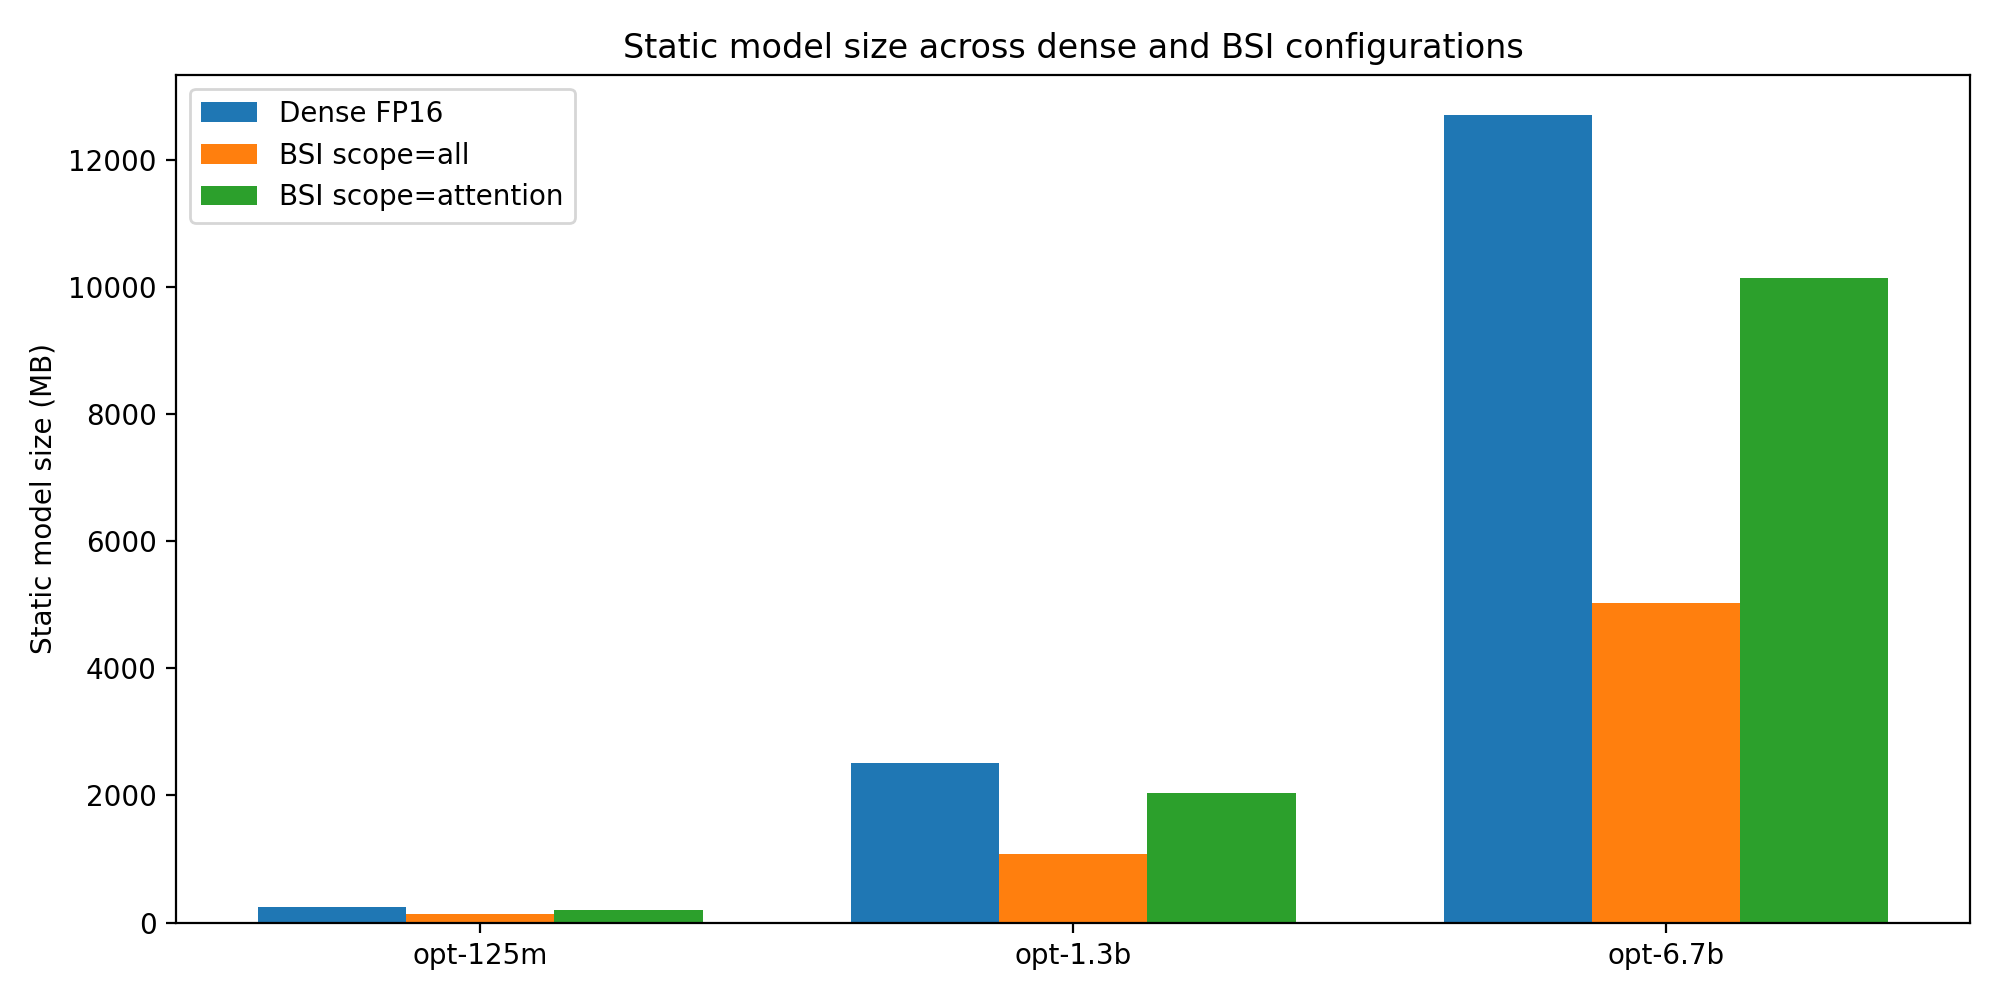
\includegraphics[width=0.9\textwidth]{memory_comparison.png}}{\fbox{\parbox{0.9\textwidth}{\centering Placeholder for a bar chart comparing dense FP16 size, BSI \texttt{scope=all} size, and BSI \texttt{scope=attention} size across OPT-125M, OPT-1.3B, and OPT-6.7B.}}}
\caption{Model static size comparison across dense and BSI configurations.}
\label{fig:memory-comparison}
\end{figure}

\begin{figure}[H]
\centering
\IfFileExists{dot_latency_comparison.png}{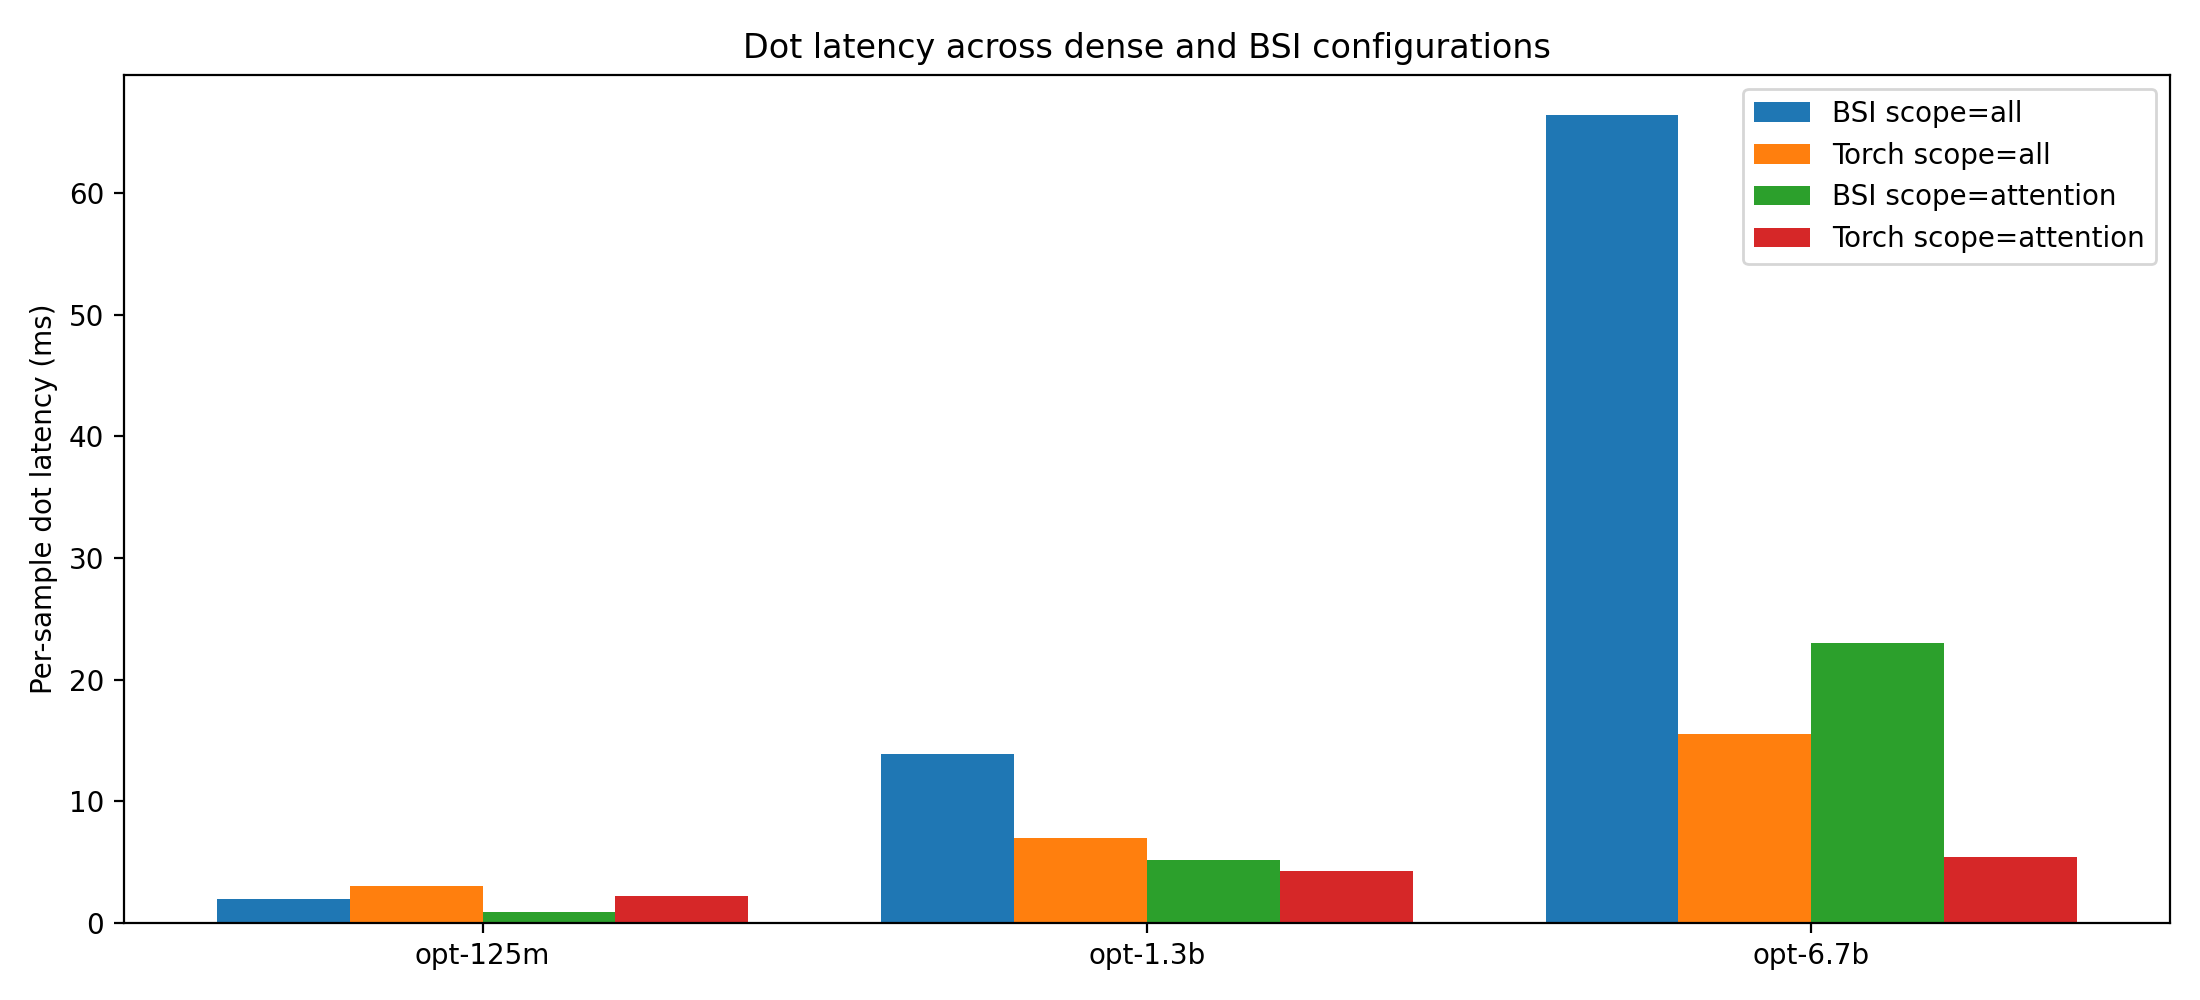
\includegraphics[width=0.9\textwidth]{dot_latency_comparison.png}}{\fbox{\parbox{0.9\textwidth}{\centering Placeholder for a grouped bar chart comparing dense Torch and BSI per-sample dot latency under \texttt{scope=all} and \texttt{scope=attention}.}}}
\caption{Per-sample dot latency comparison across models and scope policies.}
\label{fig:dot-latency-comparison}
\end{figure}

\section{Accuracy Results for \texttt{scope=all}}
\begin{table}[H]
\centering
\caption{Top-1 and Top-5 accuracy under \texttt{scope=all}.}
\label{tab:scope-all-acc}
\begin{tabular}{lrrrr}
\toprule
Model & Dense Top-1 & BSI Top-1 & Dense Top-5 & BSI Top-5 \\
\midrule
OPT-125M & 0.605 & 0.626 & 0.725 & 0.729 \\
OPT-1.3B & 0.722 & 0.653 & 0.873 & 0.796 \\
OPT-6.7B & 0.798 & 0.741 & 0.929 & 0.896 \\
\bottomrule
\end{tabular}
\end{table}

The same-bit baseline is viable on smaller models, but the accuracy gap widens as model size grows. This indicates that a uniform fixed-bit policy is not sufficient for all scales.

\section{Accuracy Results for \texttt{scope=attention}}
\begin{table}[H]
\centering
\caption{Top-1 and Top-5 accuracy under \texttt{scope=attention}.}
\label{tab:scope-attn-acc}
\begin{tabular}{lrrrr}
\toprule
Model & Dense Top-1 & BSI Top-1 & Dense Top-5 & BSI Top-5 \\
\midrule
OPT-125M & 0.605 & 0.608 & 0.725 & 0.722 \\
OPT-1.3B & 0.722 & 0.666 & 0.873 & 0.821 \\
OPT-6.7B & 0.798 & 0.779 & 0.929 & 0.921 \\
\bottomrule
\end{tabular}
\end{table}

Attention-only replacement preserves quality much better than \texttt{scope=all}, especially at larger model sizes. This is consistent with the broader conclusion that the present BSI regime is more compatible with attention projections than with the full feed-forward stack.

\begin{figure}[H]
\centering
\IfFileExists{accuracy_scope_all.png}{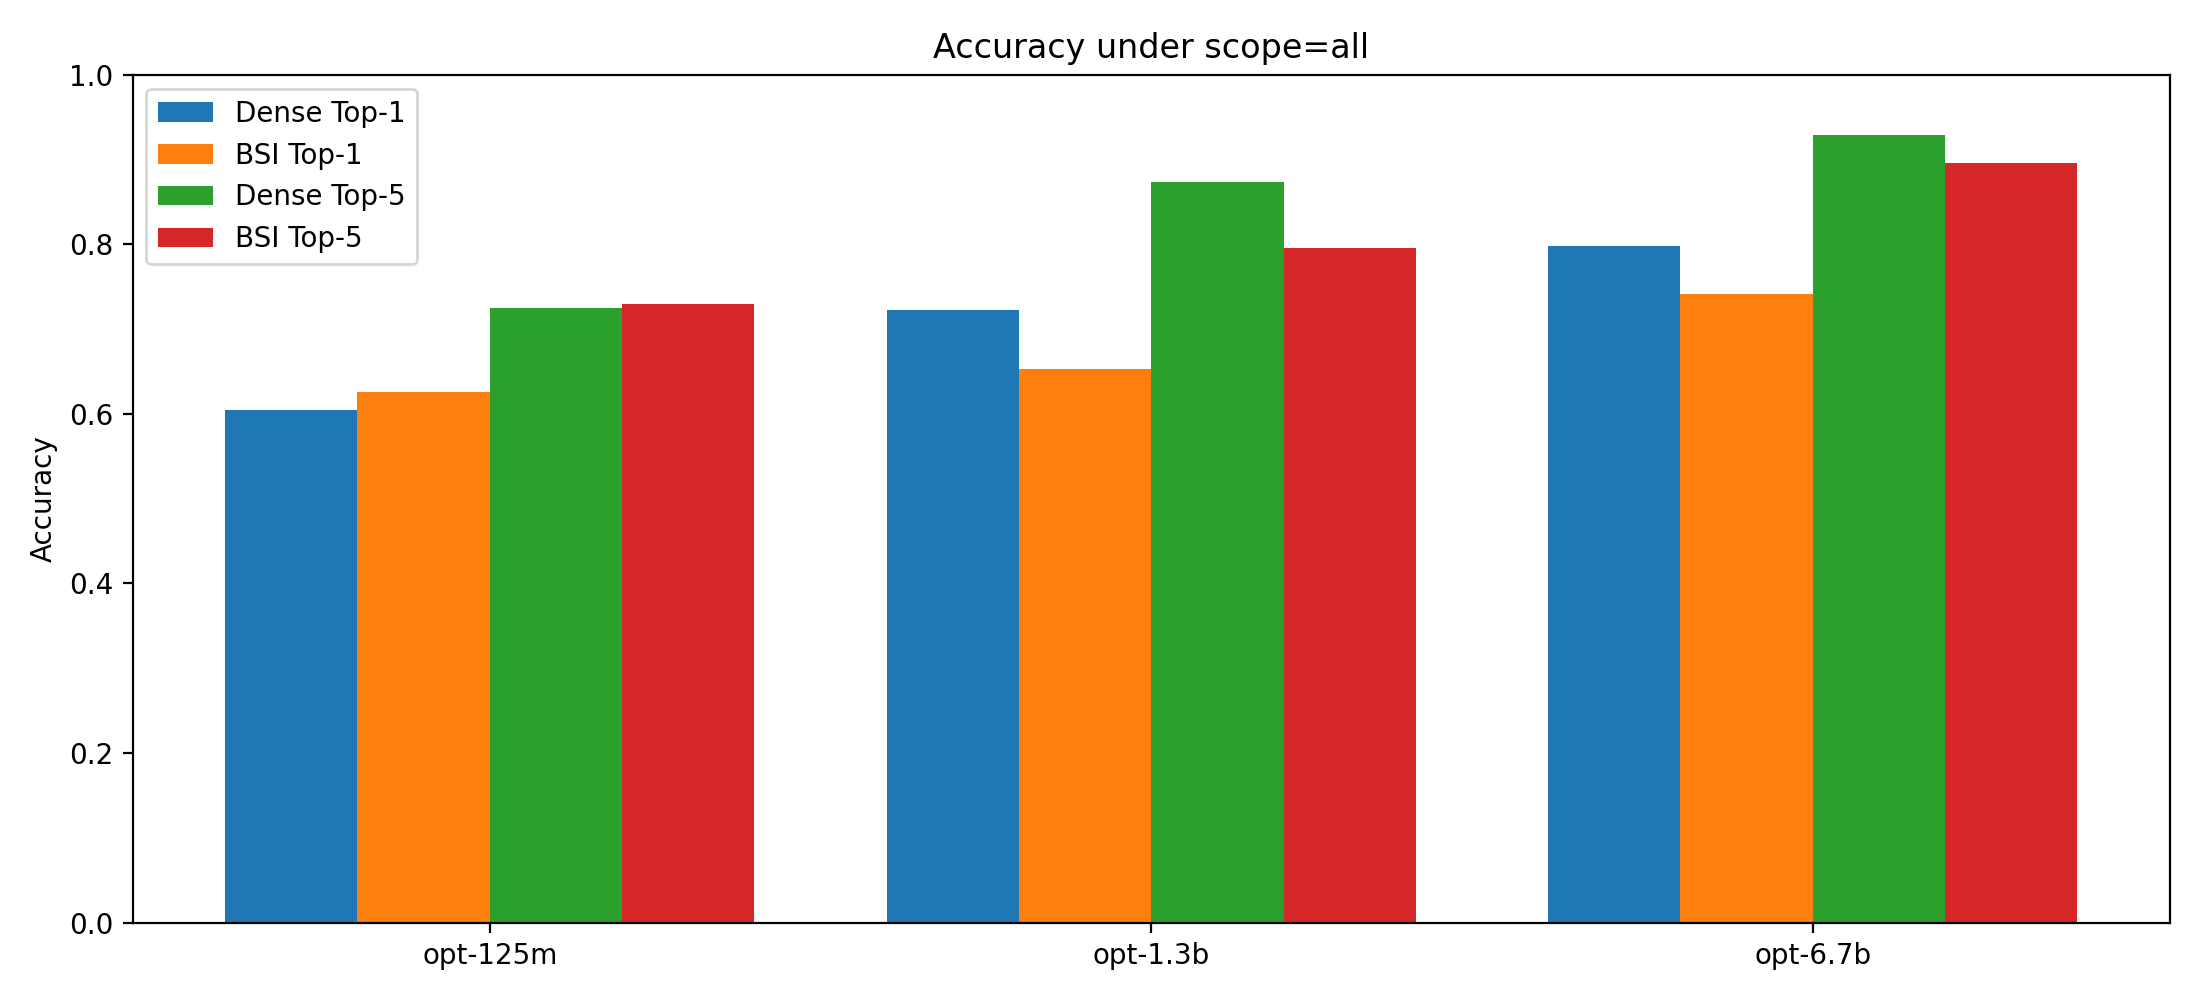
\includegraphics[width=0.9\textwidth]{accuracy_scope_all.png}}{\fbox{\parbox{0.9\textwidth}{\centering Placeholder for an accuracy plot comparing dense and BSI top-1 and top-5 results under \texttt{scope=all}.}}}
\caption{Accuracy comparison under \texttt{scope=all}.}
\label{fig:accuracy-scope-all}
\end{figure}

\begin{figure}[H]
\centering
\IfFileExists{accuracy_scope_attention.png}{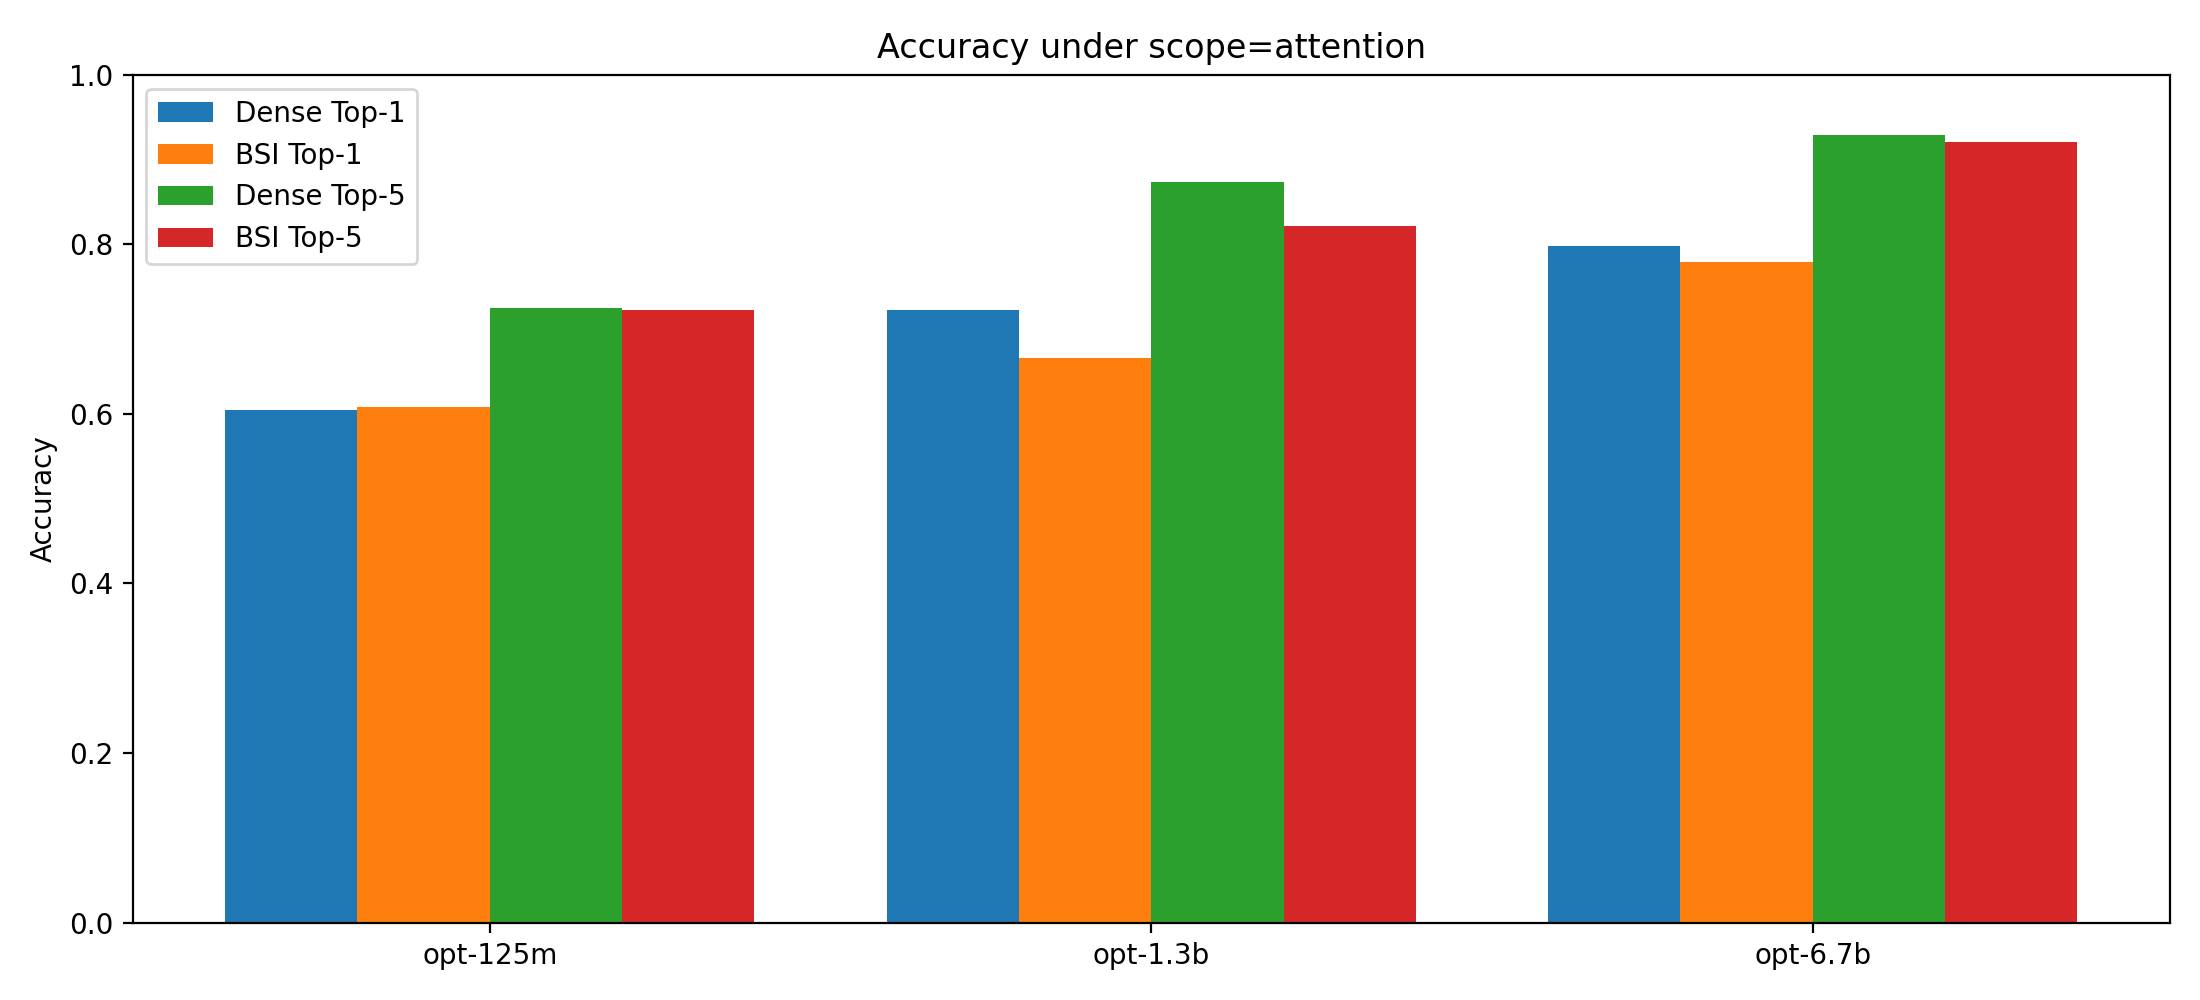
\includegraphics[width=0.9\textwidth]{accuracy_scope_attention.png}}{\fbox{\parbox{0.9\textwidth}{\centering Placeholder for an accuracy plot comparing dense and BSI top-1 and top-5 results under \texttt{scope=attention}.}}}
\caption{Accuracy comparison under \texttt{scope=attention}.}
\label{fig:accuracy-scope-attention}
\end{figure}

\section{Stable Same-Bit OPT-6.7B Case Study}
Under the primary evaluation setting, \texttt{facebook/opt-6.7b} produces the following tradeoff:
\begin{itemize}[leftmargin=2em]
\item Dense FP16: top-1 $=0.798$, top-5 $=0.929$, dot latency $=15.493$ ms, static size $=12700.031$ MB
\item BSI, \texttt{scope=all}: top-1 $=0.741$, top-5 $=0.896$, dot latency $=66.452$ ms, static size $=5022.281$ MB
\item BSI, \texttt{scope=attention}: top-1 $=0.779$, top-5 $=0.921$, dot latency $=23.003$ ms, static size $=10141.031$ MB
\end{itemize}
This case study captures the central tradeoff of the work: more aggressive BSI coverage yields better compression but a larger dot-latency penalty and a larger accuracy loss.

\chapter{Ablation Studies}

\section{Scope Ablation}
The contrast between \texttt{scope=all} and \texttt{scope=attention} is one of the most important ablations in the entire study. It shows that the present BSI regime is not uniformly compatible with all linear subgraphs of a transformer. When all eligible layers are replaced, the model achieves the largest memory reduction but also suffers the largest accuracy and latency penalties. When only attention projections are replaced, the model retains much more of the dense baseline behavior while still reducing static size and dot cost relative to full-scope BSI replacement.

This ablation matters because it establishes that the problem cannot be framed purely as a global bitwidth problem. The same bit policy has different consequences in different layer groups.

\section{Larger-Model Sensitivity}
The 30B model was used as a stress test rather than as a primary target. Its value lies in revealing how the current fixed-bit BSI policy fails.

In that model, attention-only replacement remained relatively close to the dense baseline, while MLP-only replacement degraded much more strongly. When all eligible layers were replaced, the model accuracy dropped sharply. The conclusion is direct: under the current same-bit regime, MLP layers are the dominant quality bottleneck at larger scale. This result is important because it prevents the thesis from presenting BSI quality loss as a uniform effect. The loss is structured, and that structure points directly to future work in layer-aware or subgraph-aware design.

\section{Earlier CPU-to-GPU Ablation}
The thesis also includes a broader architectural ablation that spans the two development stages of the work.

On CPU, the earlier BSI vector algebra study demonstrated that bit-sliced dot product, multiplication, and summation could be implemented correctly and could offer memory savings. However, the CPU execution cost remained too high, especially for dot product. Moving to GPU therefore was not a simple implementation convenience. It was an ablation of the execution substrate itself. The transition from CPU to GPU showed that the BSI representation had enough structure to justify further optimization, but that the representation would only be competitive if its execution path was redesigned for parallel hardware.

\section{Design Iterations that Did Not Survive}
Several aggressive design ideas were implemented and then removed after full-system testing. These negative results are important because they define the real boundary of the design space.

\subsection{Runtime Query Repacking}
One experiment repacked runtime queries into a more specialized tile layout before launching the dot kernel. That design looked plausible at the kernel level, but it increased end-to-end build cost too much. The additional runtime work outweighed the kernel-level benefit, and the design was removed from the active path. This result demonstrated that the dynamic side of the pipeline must remain simple enough to be rebuilt every layer.

\subsection{Duplicate Storage in Experimental Layouts}
Another design temporarily stored both legacy and experimental tensor formats at the same time. The result was a large increase in static model size without a proportional runtime benefit. This problem was corrected by removing duplicate storage. The lesson was straightforward: a layout experiment that ignores full-model memory accounting can easily erase the compression advantage that motivated BSI in the first place.

\subsection{Aggressive Low-Bit Frontier Points}
Lower fixed slice counts were also evaluated. Those runs reduced static size further and improved dot time, but the resulting loss in next-token accuracy was too large for them to serve as the main thesis baseline. This outcome is valuable because it clarifies the thesis argument. The work is not defending the statement that lower bits are always better. It is defending the statement that BSI performance must be studied at fixed representation quality and that the real improvements come from layout and execution design.

\section{Kernel-Tuning Ablations}
The stable same-bit configuration was reached only after several kernel-level tuning ablations. More aggressive sweep counts, alternate accumulator organizations, and alternative staging choices were tested. Some of these increased register pressure or moved cost into other parts of the pipeline without improving the end-to-end result. The validated operating point therefore should not be interpreted as arbitrary. It is the outcome of a narrowing process in which multiple plausible alternatives were rejected because they did not survive the actual model-level measurements.

\section{What the Ablations Established}
The ablation program established five conclusions.

\begin{enumerate}[leftmargin=2em]
\item The execution substrate matters: CPU BSI algebra was informative but not fast enough, which justified the move to CUDA.
\item The layer group matters: attention layers and MLP layers are not equally tolerant of the same BSI policy.
\item The dynamic side matters: a query-side optimization can still be a net loss if it must be paid at every forward pass.
\item The memory footprint matters: a kernel experiment that duplicates state is not acceptable, even if it improves a microbenchmark.
\item The arithmetic policy matters: reducing slice counts improves speed but cannot be the main result if it destroys too much accuracy.
\end{enumerate}

These conclusions are part of the thesis contribution because they define the practical constraints of native BSI inference, not just its possible benefits.

\chapter{Discussion}
\section{What Was Achieved}
The work achieved a full BSI-native inference pipeline for OPT-family models, a functioning CUDA builder for weights and activations, a stable same-bit tensor-core baseline on Hopper-class hardware, and a benchmark harness that separates kernel-only, layer-level, and end-to-end behavior. It also established a clear compression/accuracy/performance tradeoff across scope policies and model sizes.

\section{What Must Be Defended}
The defensible thesis argument is not that BSI already surpasses dense Torch inference. The defensible argument is that BSI becomes materially more viable only when representation and execution are designed together. The implementation and the measurements support that claim by showing that naive bit-sliced execution is slow, that some layout-aware changes help, and that the remaining gap is now well explained by profiler evidence.

\section{What Was Not Achieved}
Several things should not be overstated. The BSI dot kernel does not yet match dense FP16 throughput. The current fixed-bit regime does not scale cleanly to the 30B model under \texttt{scope=all}. Lower slice counts improve speed but do not preserve enough accuracy to serve as the main thesis result. These limitations do not invalidate the work, but they define its scope clearly.

\chapter{Future Work}
The next research steps follow directly from the profiler evidence and the scope-ablation results.
\begin{enumerate}[leftmargin=2em]
\item Redesign the arithmetic formulation so that the effective slice interaction count is reduced without abandoning BSI-native execution.
\item Develop shape-specialized kernels for attention projections, FC1, and FC2 rather than relying on one general stable point.
\item Introduce layer-aware or subgraph-aware bit policies, especially for MLP layers.
\item Redesign shared-memory layouts to reduce bank conflicts and excessive wavefronts.
\item Extend the evaluation beyond OPT and beyond LAMBADA-only scoring.
\item Calibrate the documentation pipeline further by converting profiler captures and benchmark tables into publication-ready figures automatically.
\end{enumerate}

\chapter{Conclusion}

This work establishes a complete path from bitmap-based BSI algebra to GPU-based large language model inference. The earlier CPU stage showed that bit-sliced vectors could represent numeric data compactly, support a richer algebra than simple storage, and preserve control over precision and sparsity. It also showed that CPU execution was not sufficient to make those benefits practical for large neural-network workloads. That limitation motivated the transition to CUDA.

The GPU stage preserved the BSI semantics and scaled them into a transformer inference pipeline. Static weights were converted into BSI key structures, dynamic activations were converted into batched query slices, and the dominant matrix products in OPT models were executed through same-bit CUDA dot kernels. The resulting system provides substantial compression, a functioning end-to-end inference path, and a stable operating point across \texttt{opt-125m}, \texttt{opt-1.3b}, and \texttt{opt-6.7b}.

The results make the main thesis argument defensible. BSI can be used as a native compressed representation for LLM inference on GPUs, but only when representation and kernel execution are designed together. Compression alone is not enough. Lower bit count alone is not enough. The data layout, the runtime build path, and the structure of the dot kernel determine whether the representation becomes practically useful.

At the same time, the study is clear about what remains unresolved. The stable same-bit dot path still trails dense FP16 Torch execution by a large margin on larger models. Full-scope replacement also becomes increasingly sensitive as model size grows, with feed-forward layers emerging as a major quality bottleneck. These limits do not weaken the thesis. They define the current frontier precisely.

The thesis therefore closes with a clear systems conclusion: the feasibility of BSI-native transformer inference has been established, the primary tradeoffs are now measured, and the next stage of research is sharply defined. The remaining challenge is to redesign the arithmetic and layout of the BSI dot path so that the representation keeps its compression advantage while scaling much more efficiently on GPU hardware.


\appendix
\chapter{Reproducibility Commands}
\section{Cluster and Environment Setup}
The following commands assume that the repository has already been cloned and that execution starts from the repository root.

\begin{verbatim}
source bsi_ops/network_connection.sh
module load nvhpc-hpcx-cuda12/24.11
source gpu_connection.sh          # if your cluster provides this helper
source gpu_env_setup.sh
git submodule update --init --recursive
source /home/017510883/miniconda3/bin/activate bsiPytorch
cd bsi_ops
bash rebuild_local.sh
\end{verbatim}

\section{Repository Setup}
\begin{verbatim}
git clone https://github.com/gguzunsjsu/bsiPytorch.git
cd bsiPytorch
\end{verbatim}

\section{Stable Same-Bit Environment}
\begin{verbatim}
export BSI_TC_DOT=1
export BSI_TC_FIXED_INT=1
export BSI_TC_CPASYNC=1
export BSI_TC_TM=32
export BSI_FIXED_BITS_KEYS=6
export BSI_FIXED_BITS_QUERIES=7
export BSI_FIXED_CHUNK_SCALE=1
export BSI_TC_R_SWEEP=4
export BSI_TC_TMA=1
export BSI_DOT_DEBUG=1   # optional
\end{verbatim}

\section{Kernel-Only Commands}
\begin{verbatim}
python benchmarks/benchmark_apples_to_apples_bsi.py --modes kernel_only \
  --Q 512 --R 16384 --D 4096 \
  --decimal_places 2 --compress_threshold 0.5 \
  --torch_dtype fp16 --bsi_profile 0 --base_dtype fp16

python benchmarks/benchmark_apples_to_apples_bsi.py --modes kernel_only \
  --Q 512 --R 50272 --D 4096 \
  --decimal_places 2 --compress_threshold 0.5 \
  --torch_dtype fp16 --bsi_profile 0 --base_dtype fp16
\end{verbatim}

\section{Model End-to-End Command}
\begin{verbatim}
python benchmarks/benchmark_apples_to_apples_bsi.py --modes model_e2e \
  --model_name facebook/opt-6.7b \
  --dataset lambada --split validation --num_samples 200 \
  --decimal_places 2 --compress_threshold 0.5 \
  --scope all --bsi_device cuda --bsi_profile 1 --base_dtype fp16
\end{verbatim}

\section{Nsight Compute Commands}
\begin{verbatim}
ncu --set full --target-processes all -f -o ncu_rsweep4_tma_fc1 \
  -k popcount_weighted_keys_literal_fused_bmma_tc_kernel_tm32_fixed76_chunkscale_rsweep4_tma_tensorB \
  --launch-count 1 \
  python benchmarks/benchmark_apples_to_apples_bsi.py --modes kernel_only \
    --Q 512 --R 16384 --D 4096 \
    --decimal_places 2 --compress_threshold 0.5 \
    --warmup 0 --iters 1 --torch_dtype fp16 --bsi_profile 0 --base_dtype fp16

ncu --set full --target-processes all -f -o ncu_rsweep4_tma_vocab \
  -k popcount_weighted_keys_literal_fused_bmma_tc_kernel_tm32_fixed76_chunkscale_rsweep4_tma_tensorB \
  --launch-count 1 \
  python benchmarks/benchmark_apples_to_apples_bsi.py --modes kernel_only \
    --Q 512 --R 50272 --D 4096 \
    --decimal_places 2 --compress_threshold 0.5 \
    --warmup 0 --iters 1 --torch_dtype fp16 --bsi_profile 0 --base_dtype fp16

BSI_TC_TMA=0 ncu --set full --target-processes all -f -o ncu_rsweep4_no_tma \
  -k popcount_weighted_keys_literal_fused_bmma_tc_kernel_tm32_fixed76_chunkscale_rsweep4 \
  --launch-count 1 \
  python benchmarks/benchmark_apples_to_apples_bsi.py --modes kernel_only \
    --Q 512 --R 16384 --D 4096 \
    --decimal_places 2 --compress_threshold 0.5 \
    --warmup 0 --iters 1 --torch_dtype fp16 --bsi_profile 0 --base_dtype fp16
\end{verbatim}

\section{Figure Generation Commands}
\begin{verbatim}
python docs/latex/scripts/generate_benchmark_plots.py
bash docs/latex/scripts/stage_ncu_screenshots.sh docs/latex/figures/raw docs/latex/figures/manual
\end{verbatim}


\bibliographystyle{plain}
\bibliography{latex/references}

\end{document}
